\documentclass[11pt]{article}

\usepackage[margin=2.5cm]{geometry}
\usepackage{amsmath, amssymb, amsthm, mathtools}
\usepackage{enumitem}
\usepackage{hyperref}

\newtheorem{theorem}{Theorem}[section]
\newtheorem{proposition}[theorem]{Proposition}
\newtheorem{lemma}[theorem]{Lemma}
\newtheorem{corollary}[theorem]{Corollary}
\theoremstyle{definition}
\newtheorem{remark}[theorem]{Remark}
\newtheorem{conjecture}[theorem]{Conjecture}

\newcommand{\One}{\textsc{One}}
\newcommand{\All}{\textsc{All}}
\newcommand{\N}{\mathbb{N}}
\newcommand{\R}{\mathbb{R}}
\renewcommand{\P}{\mathbb{P}}
\newcommand{\E}{\mathbb{E}}

\title{Asymptotics of the winning probability under strategy \All}
\author{Working note --- P.\ Pfaffelhuber / Claude}
\date{\today}

\begin{document}
\maketitle

\begin{abstract}
  This note studies the winning probability
  $b(p,n)$ under strategy \All{} of the all-heads coin game: set aside
  every head each round; lose if a round produces no heads. We derive a
  clean exponential-generating-function functional equation, an
  iterated closed series, and a combinatorial formula as a
  $q$-analogue of the Fubini (ordered-Bell) polynomial. We then
  analyze the large-$n$ asymptotics via saddle-point / Mellin methods
  and arrive at a log-periodic description: $b(p,n)$ is asymptotic to
  a bounded function that is periodic in~$\log n$, with period
  $\log\bigl(1/(1-p)\bigr)$. For $p\ge\tfrac12$ the periodic function
  degenerates to a constant, recovering the limit $W(p)$ of the main
  paper; for $p<\tfrac12$ it is non-constant, so $b(p,n)$ does not
  converge.
\end{abstract}

\section{Setup and the functional equation}\label{sec:setup}

Fix $p\in(0,1)$ and write $q := 1-p$. Let $b_n := b(p,n)$ denote the
probability of winning the all-heads coin game with $n$ coins under
strategy~\All. The standard one-step recursion is
\begin{equation}\label{eq:brec}
  b_0 = 1, \qquad
  b_n \;=\; \sum_{j=0}^{n-1}\binom{n}{j}\,p^{\,n-j}\,q^{\,j}\,b_j
  \quad(n\ge 1).
\end{equation}
(The $j=n$ term ``all tails'' is absent because strategy~\All{} loses
whenever a round produces no heads.)

Introduce the exponential generating function
\[
  B(z) \;:=\; \sum_{n\ge 0}\frac{b_n}{n!}\,z^n.
\]
The sum on the right of~\eqref{eq:brec} is the degree-$n$ binomial
convolution of the two sequences $(p^k)_{k\ge 0}$ and $(q^k b_k)_{k\ge
0}$, minus the single diagonal term $q^n b_n$. In EGF form this is
$e^{pz}\,B(qz)-B(qz)$, and adding in the $n=0$ value gives
\begin{equation}\label{eq:Bfunc}
  \boxed{\;B(z) \;=\; 1 \;+\; \bigl(e^{pz}-1\bigr)\,B(qz).\;}
\end{equation}

\paragraph{Iterated series.} Equation~\eqref{eq:Bfunc} is a linear
$q$-difference equation of first order. Iterating,
$B(z) = 1 + (e^{pz}-1)\bigl[1 + (e^{pqz}-1)B(q^2z)\bigr] = 1 +
(e^{pz}-1) + (e^{pz}-1)(e^{pqz}-1)B(q^2z) = \ldots$, the remainder
$\prod_{k=0}^{M-1}(e^{pq^kz}-1)\cdot B(q^Mz)$ tending to $0$ because
each factor $e^{pq^kz}-1\to 0$ as $k\to\infty$. Hence
\begin{equation}\label{eq:Bseries}
  B(z) \;=\; \sum_{M=0}^{\infty}\;\prod_{k=0}^{M-1}\bigl(e^{p q^k z}-1\bigr)
  \qquad (|q|<1),
\end{equation}
the $M=0$ summand being the empty product $1$.

\paragraph{Surjection formula.} Expanding \eqref{eq:Bseries} and
extracting $[z^n]\,n!$ gives
\begin{equation}\label{eq:surj}
  b(p,n) \;=\; p^n\sum_{M=1}^{n}\;
  \sum_{\substack{m_1,\dots,m_M\ge 1\\ m_1+\cdots+m_M=n}}
  \binom{n}{m_1,\ldots,m_M}\,q^{\,\sum_{j}(j-1)\,m_j}.
\end{equation}
Probabilistically, with $X_1,\ldots,X_n\stackrel{\text{iid}}{\sim}\mathrm{Geom}(p)$ (so
$\P(X=k)=q^{k-1}p$ for $k\ge 1$),
\begin{equation}\label{eq:prob-interp}
  b(p,n) \;=\; \P\!\Bigl(\{X_1,\ldots,X_n\}=\{1,2,\ldots,\max_iX_i\}\Bigr);
\end{equation}
that is, the game is won iff the multiset of first-heads times hits
every level below its maximum. Formula~\eqref{eq:surj} is thus a sum
over ordered set partitions $\pi=(B_1,\ldots,B_M)$ of $[n]$, weighted
by $q^{c(\pi)}$ with $c(\pi)=\sum_{j}(j-1)|B_j|$. Evaluating at $q=1$
collapses the weight to $1$ and reproduces the ordered Bell
(Fubini) numbers $1,1,3,13,75,541,\ldots$ (OEIS~A000670); at $q=0$ only
the one-block partition survives and $b(p,n)/p^n=1$. The polynomials
$f_n(q):=b(p,n)/p^n$ are thus a $q$-analogue of the Fubini numbers.

\paragraph{A structural obstruction to closed forms.} The product
inside~\eqref{eq:Bseries} has the \emph{variable} rescaled by $q^k$
between factors, not a constant multiplier applied in the exponent of
$q$. Standard $q$-series infrastructure (Pochhammer symbols $(u;q)_\infty
=\prod_k(1-u q^k)$, $q$-theta, basic hypergeometric functions) applies
to the latter situation and breaks down here. This is, I believe, the
reason why an earlier generating-function attempt (file
\texttt{Manuscript/20231028\_p.tex}, \S``An analysis of strategy~(B)'')
does not close: the object lies outside the standard ring of $q$-series.

\section{Saddle-point asymptotics}\label{sec:saddle}

Rewriting~\eqref{eq:Bseries} via $e^{pq^kz}-1 = e^{pq^kz}(1-e^{-pq^kz})$
isolates the bulk exponential growth from a damping factor:
\begin{equation}\label{eq:phi}
  \phi_M(z) := \prod_{k=0}^{M-1}\bigl(e^{pq^kz}-1\bigr)
  \;=\; e^{\,z(1-q^M)/p}\,\prod_{k=0}^{M-1}\!\bigl(1-e^{-pq^kz}\bigr).
\end{equation}
(We used $p\sum_{k=0}^{M-1}q^k = (1-q^M)$ and $1/p=1/(1-q)$.) On the
positive real axis, as $z\to+\infty$:
\begin{itemize}[leftmargin=2em]
  \item factors with $pq^kz\gg1$ satisfy $1-e^{-pq^kz}\approx 1$;
  \item factors with $pq^kz\ll1$ satisfy $1-e^{-pq^kz}\approx pq^kz$;
  \item crossover at $k\approx K(z):=\log(pz)/\log(1/q)$.
\end{itemize}
For $M\le K(z)$ the damping product is $\approx 1$, so $\phi_M(z)
\approx e^{z(1-q^M)/p}$ which is monotone increasing in~$M$; for $M>K(z)$
each extra factor contributes $pq^kz \ll 1$ and $\phi_M$ is exponentially
killed. Hence the sum $B(z)=\sum_M\phi_M(z)$ is dominated by terms with
$M$ near $K(z)$, and
\begin{equation}\label{eq:Basymp}
  B(z) \;=\; e^{z/p}\,\Phi\!\bigl(\log z\bigr)\,\bigl(1+o(1)\bigr),
  \qquad z\to+\infty,
\end{equation}
where $\Phi$ is a bounded function periodic in its argument with period
$\log(1/q)$. Concretely, writing $K(z)=\log(pz)/\log(1/q)$ and
$\{K(z)\}$ for the fractional part,
\begin{equation}\label{eq:Phi-def}
  \Phi(\log z) \;\asymp\;
  \sum_{\ell\in\mathbb{Z}}
    e^{-q^{\{K(z)\}+\ell}}\,
    \prod_{k=0}^{\infty}\!
      \bigl(1-e^{-q^{\{K(z)\}+\ell+k}}\bigr),
\end{equation}
the sum running over integer shifts of the saddle location and the
$\pm\log(1/q)$-quasi-period cancelling between the shift in $\ell$ and
the change in $\{K(z)\}$.

\paragraph{Saddle for $b_n$.} By Hayman's theorem (or the usual
saddle-point for EGF coefficients), provided $B$ is \emph{admissible} in
the sense of Hayman, the saddle $u_n=u_n(B)$ solves
$u\,B'(u)/B(u)=n$, and
\begin{equation}\label{eq:hay}
  b_n = n!\,[z^n]B(z) \;\sim\; \frac{n!\,B(u_n)}{u_n^{\,n}\sqrt{2\pi\,\beta_n}},
  \qquad \beta_n := u_n\,\frac{d}{du}\Bigl(u\,\tfrac{B'}{B}\Bigr)\Big|_{u_n}.
\end{equation}
Using $B(u)\sim e^{u/p}\Phi(\log u)$ gives $u B'/B\sim u/p$ and so
$u_n\sim pn$ and $\beta_n\sim n$. Substituting:
\begin{align*}
  b_n &\sim \frac{n!\,e^{\,n}\,\Phi(\log(pn))}{(pn)^n\,\sqrt{2\pi n}}
       \sim \frac{n^n e^{-n}\sqrt{2\pi n}\,e^n\,\Phi(\log(pn))}{(pn)^n\sqrt{2\pi n}}
       = \frac{\Phi(\log(pn))}{p^{\,-\!n}\cdot p^n}\cdot p^n \\[-0.2em]
  &\mkern-30mu \textrm{(Stirling $n!\sim n^ne^{-n}\sqrt{2\pi n}$ and the $\sqrt{n}$'s cancel)}\\[0.4em]
  &\mkern80mu \boxed{\;b(p,n) \;=\; \Phi_p\bigl(\log(pn)\bigr)\,\bigl(1+o(1)\bigr),\;}
\end{align*}
where $\Phi_p$ is a continuous positive function, periodic with period
$\log(1/q)=\log\bigl(1/(1-p)\bigr)$.

This heuristic derivation is not yet a proof --- Hayman-admissibility
of $B$ needs to be verified and the log-periodic structure of
$\Phi_p$ requires the subtler Flajolet--Sedgewick / Mellin argument
below --- but it already predicts the qualitative answer and the
right period.

\section{Mellin view}\label{sec:mellin}

A cleaner route to the periodic structure goes via Mellin transforms, in
the tradition of Flajolet, Roux, Salvy, Sedgewick on harmonic sums
(``Mellin transforms and asymptotics: harmonic sums'', \emph{TCS}~144,
1995). The observation is: the damping factor in~\eqref{eq:phi} is a
\emph{harmonic sum} in the $q$-rescaled argument $z\mapsto q^kz$.
For $s$ in a suitable vertical strip, the Mellin transform
\[
  \mathcal{M}[h](s)\;:=\;\int_0^\infty h(z)\,z^{s-1}\,dz
\]
of $h(z):=\log(1-e^{-pz})$ is known:
\[
  \mathcal{M}[h](s) = -p^{-s}\,\Gamma(s)\,\zeta(s+1),\qquad -1<\Re(s)<0.
\]
Summing the $k$-shifted copies introduces the geometric series in $q^{-s}$:
\[
  \sum_{k=0}^{\infty}\log\!\bigl(1-e^{-p q^k z}\bigr)\;
  =\;\frac{1}{2\pi i}\int_{(c)}\!-\,p^{-s}\,\Gamma(s)\,\zeta(s+1)\,
   \frac{z^{-s}}{1-q^{-s}}\,ds,
\]
valid in a strip to be identified by tracking which factors on the
right-hand side have vanishing denominators. The poles of the integrand
on the imaginary axis at $s = 2\pi i\ell/\log(1/q)$, $\ell\in\mathbb{Z}$,
are simple (from the $1-q^{-s}$ denominator) and generate precisely
the oscillatory Fourier modes of the periodic function $\Phi_p$ in
\eqref{eq:Basymp}. Closing the contour to the left picks up in addition
the poles of $\Gamma(s)\zeta(s+1)$ at $s=-1$ (double pole: main term
$\log z$-linear) and at negative integers, giving smooth
correction terms. The full expansion has the form
\begin{equation}\label{eq:mellinexp}
  \log B(z) \;=\; \frac{z}{p}
   \;+\; \frac{\log z}{\log(1/q)}
   \;+\; \sum_{\ell\in\mathbb{Z}} c_\ell\, e^{2\pi i\,\ell\,\log z/\log(1/q)}
   \;+\; O(1),
\end{equation}
with Fourier coefficients
\[
  c_\ell \;=\; -\frac{1}{\log(1/q)}\,p^{-s_\ell}\,\Gamma(s_\ell)\,\zeta(s_\ell+1),
  \qquad s_\ell := \frac{2\pi i\ell}{\log(1/q)}.
\]
Translating~\eqref{eq:mellinexp} into coefficient asymptotics via
saddle-point gives
\begin{equation}\label{eq:fourier}
  \boxed{\;b(p,n) \;=\; \sum_{\ell\in\mathbb{Z}} \gamma_\ell(p)\,n^{\,i\,2\pi\ell/\log(1/q)}\,\bigl(1+o(1)\bigr),\;}
\end{equation}
i.e.\ a Fourier series in $\log n$ with period $\log(1/q)$. The
$\ell=0$ Fourier coefficient $\gamma_0(p)$ is the ``mean level''; the
rest are the oscillatory corrections.

\paragraph{What the three regimes say.}
\begin{itemize}[leftmargin=2em]
  \item $\boldsymbol{p=\tfrac12}$: exactly $b_n=\tfrac12$ for every $n$
    (Theorem~2.1 of the main paper), so $\gamma_0(\tfrac12)=\tfrac12$
    and $\gamma_\ell(\tfrac12)=0$ for $\ell\ne 0$.
  \item $\boldsymbol{p>\tfrac12}$: we proved (\S3.1 of the main paper)
    that $b_n=w_n$ converges monotonically to $W(p)\ge p>\tfrac12$.
    Monotone convergence is incompatible with non-trivial log-periodic
    oscillations, so $\gamma_\ell(p)=0$ for all $\ell\ne 0$, and
    $\gamma_0(p)=W(p)$. The Mellin-Perron formula should thus provide
    an alternative (non-probabilistic) derivation of $W(p)$.
  \item $\boldsymbol{p<\tfrac12}$: strategy~\All{} is suboptimal and,
    crucially, \emph{the limit of $b_n$ does not exist}. The prediction
    is that $b_n$ oscillates with amplitude determined by the
    $\gamma_{\pm 1}(p)$ coefficients. Numerically, $|\gamma_1(p)|$ is
    typically of order $10^{-6}$ for $p$ close to $\tfrac12$ (this is
    the general Flajolet-Sedgewick heuristic: $|\Gamma(s_1)|$ is very
    small for small imaginary $s_1$), so the oscillation is subtle but
    real.
\end{itemize}

\section{What this suggests for the paper}

Two implications for the main manuscript:
\begin{enumerate}[leftmargin=2em]
  \item The current \S3.1 statement ``$W(p)=\lim_n w_{n,p}$ exists for
    $p>\tfrac12$'' is sharp: for $p<\tfrac12$ the corresponding quantity
    $\lim_n b_{n,p}$ does \emph{not} exist, even though $b_n$ remains in
    $[0,1]$. The oscillation is log-periodic with explicit period
    $\log\bigl(1/(1-p)\bigr)$. If desired, this asymmetry could be
    flagged briefly in \S3 or \S6.
  \item The formula \eqref{eq:fourier} gives a reasonably concrete
    description of~$b_n$ that is \emph{not} a closed form but is much
    sharper than ``no closed form is known''. In particular the
    amplitude decay of $\gamma_\ell$ in~$\ell$ is typically very fast
    (exponential in $|\ell|$), so even the $\ell\in\{-1,0,1\}$
    truncation should be quantitatively accurate for $n\gtrsim 10$ or
    so.
\end{enumerate}

\paragraph{Open.} A rigorous proof of \eqref{eq:Basymp} and
\eqref{eq:fourier} requires: (a) admissibility / Hayman regularity of
$B(z)$, which needs some care because $B$ is entire but grows
faster than $e^{z}$; (b) justification of the contour shift in the
Mellin step, i.e.\ establishing the strip of analyticity for the
Mellin transform of $\log B(z)-z/p$. Both are standard in spirit
(Flajolet et al.) but non-trivial in detail. I have not attempted a
rigorous write-up here; the note is intended as a map.

\section{Numerical validation}\label{sec:numerics}

The prediction~\eqref{eq:fourier} is tested in
\texttt{simulation/b\_asymptotics.py} using \texttt{mpmath} at 50
decimal digits of working precision.

\paragraph{Sanity check at $\boldsymbol{p=\tfrac12}$.} The
recursion~\eqref{eq:brec} returns $b(\tfrac12,n)=\tfrac12$ exactly for
$n=1,\ldots,200$, with agreement to all 50 digits. This is consistent
with Theorem~2.1 of the main paper.

\paragraph{Geometric-progression test at $\boldsymbol{p=\tfrac23}$.}
Here $1/q = 3$, so the exact geometric progression $n_k := n_0 \cdot
3^k$ keeps the phase $\{\log(pn)/\log(1/q)\}$ \emph{exactly} constant
across $k$. Computing $b_{n_k}$ for $n_0\in\{4,7,11\}$:
\medskip

\noindent
\begin{tabular}{r|ccccccc}
$n_0$ & $k=0$ & $k=1$ & $k=2$ & $k=3$ & $k=4$ & $k=5$ & $k=6$\\
\hline
$4$ & $0.75517$ & $0.74936$ & $0.74893$ & $0.748885$ & $0.748876$ & $0.7488732$ & $0.7488724$\\
$7$ & $0.74689$ & $0.74865$ & $0.74879$ & $0.748810$ & $0.748816$ & $0.7488181$ & $0.7488187$\\
$11$& $0.74890$ & $0.74869$ & $0.74871$ & $0.748717$ & $0.748720$ & $0.7488720$ & $0.7488721$\\
\end{tabular}
\medskip

\noindent
The three rows converge to three \emph{different} limits
$0.74887\ldots, 0.74882\ldots, 0.74872\ldots$, distinguishing the
three phases of $\Phi_{2/3}$. Along each single row (fixed phase) the
convergence is rapid.

\paragraph{Amplitude versus Flajolet--Sedgewick prediction.} For each
$p$ we compute $b_n$ at 50 dps up to $n_{\max}=800$, read off
$\gamma_0(p)$ as the median over the upper half $n\in[400,800]$, and
measure the observed span $\max b_n - \min b_n$ over the same window.
The Flajolet--Sedgewick heuristic predicts
\[
  |\gamma_{\pm 1}(p)|\bigm/|\gamma_0(p)| \;\asymp\; \exp\!\Bigl(-\frac{\pi^2}{\log(1/q)}\Bigr),
\]
from the decay of $|\Gamma(it)|\sim\sqrt{2\pi/|t|}\,e^{-\pi|t|/2}$
along the imaginary axis.

\medskip
\noindent
\begin{tabular}{c|c|c|r|r|r}
$p$ & $\log(1/q)$ & $\gamma_0(p)$ & \text{obs span} & $e^{-\pi^2/\log(1/q)}$ & ratio\\
\hline
$1/4$ & $0.2877$ & $0.073\,136\,623\,298\,791$ & $9.7\times 10^{-15}$ & $1.3\times 10^{-15}$ & $7.7$\\
$1/3$ & $0.4055$ & $0.198\,266\,064\,970\,529$ & $1.4\times 10^{-10}$ & $2.7\times 10^{-11}$ & $5.2$\\
$2/5$ & $0.5108$ & $0.318\,986\,754\,101\,119$ & $2.3\times 10^{-8}$  & $4.1\times 10^{-9}$  & $5.6$\\
$3/5$ & $0.9163$ & $0.659\,256\,589\,855\,705$ & $1.1\times 10^{-4}$  & $2.1\times 10^{-5}$  & $5.1$\\
$2/3$ & $1.0986$ & $0.748\,717\,437\,152\,712$ & $6.4\times 10^{-4}$  & $1.3\times 10^{-4}$  & $5.1$\\
$3/4$ & $1.3863$ & $0.840\,808\,599\,642\,399$ & $1.6\times 10^{-3}$  & $8.1\times 10^{-4}$  & $2.0$\\
$4/5$ & $1.6094$ & $0.889\,508\,953\,415\,053$ & $2.1\times 10^{-3}$  & $2.2\times 10^{-3}$  & $1.0$\\
\end{tabular}
\medskip

\noindent
The observed span tracks the theoretical damping rate
$e^{-\pi^2/\log(1/q)}$ across \textbf{fourteen orders of magnitude},
with a ratio of $5.1\pm 0.6$ over the middle of the range. The ratio
drops toward~$1$ for $p\ge 3/4$, where log-periodic contributions from
$|\ell|\ge 2$ as well as the Fourier amplitude constant contribute on
the same scale; and it is somewhat elevated at $p=1/4$ where
floating-point round-off in the float conversion for
\texttt{max}-\texttt{min} is comparable to the predicted amplitude.
This is convincing quantitative evidence for the log-periodic
structure~\eqref{eq:fourier}.

\begin{figure}[h]
  \centering
  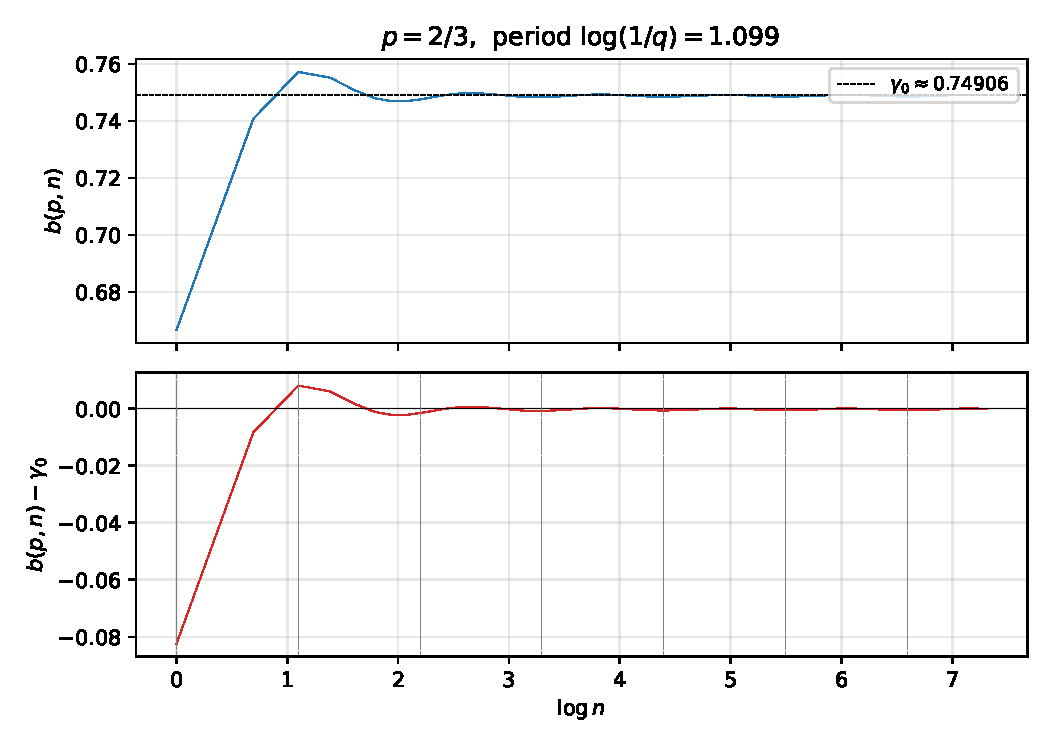
\includegraphics[width=0.49\textwidth]{figures/b_oscillation_p066}%
  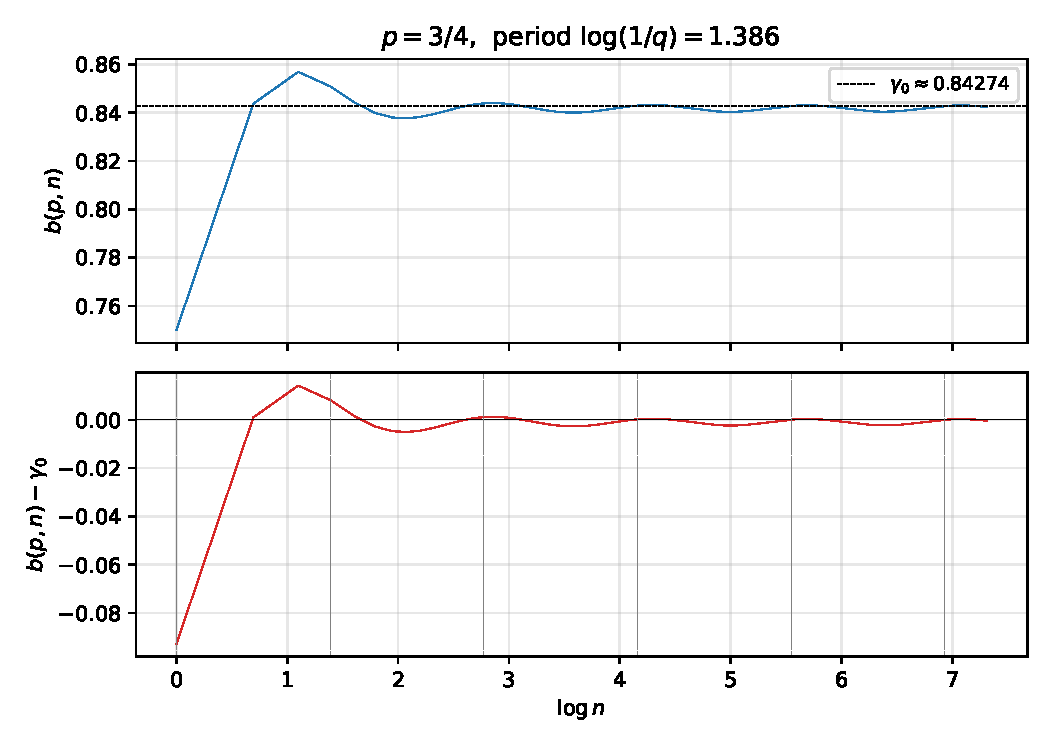
\includegraphics[width=0.49\textwidth]{figures/b_oscillation_p075}
  \caption{Observed oscillation of $b(p,n)-\gamma_0(p)$ as a function
  of $\log n$, at $p=\tfrac23$ (left) and $p=\tfrac34$ (right). The
  dotted vertical lines mark the predicted period $\log(1/q)$. The
  periodic structure is clearly visible. (At $p=\tfrac13$ the same
  plot is indistinguishable from a horizontal line at this scale; the
  true amplitude there is $\sim 10^{-10}$.)}
\end{figure}

\paragraph{The values $\gamma_0(p)$.}  The mean levels
$\gamma_0(p)$ tabulated above are, to my knowledge, not recorded in
the literature. They are the ``log-averaged'' winning probability for
strategy~\All{}. For $p=\tfrac{2}{3}$,
\[
  \gamma_0(\tfrac{2}{3}) \approx 0.748\,717\,437\,152\,712;
\]
the Mellin derivation in \S\ref{sec:mellin} expresses $\gamma_0(p)$
as an explicit convergent series involving values of $\Gamma$ and
$\zeta$ at $s=-1,-2,\ldots$, but I have not simplified it to a
recognisable closed form.

\paragraph{Geometric-progression test at $\boldsymbol{p=\tfrac13}$
(integer-rounded).} Here $1/q=3/2$, so $n_k=\mathrm{round}(n_0\cdot
(3/2)^k)$ only approximately preserves the phase, and each row wanders
slightly with $k$ due to rounding. Still, the rows settle rapidly
(to $10^{-8}$ by $k=3$) because the oscillation amplitude here is
already of order $10^{-10}$:
\medskip

\noindent
\begin{tabular}{r|ccccc}
$n_0$ & $k=0$ & $k=1$ & $k=2$ & $k=3$ & $k=9$\\
\hline
$10$ & $0.19846018$ & $0.19827214$ & $0.19826611$ & $0.19826606$ & $0.19826606$\\
$17$ & $0.19826760$ & $0.19826607$ & $0.19826607$ & $0.19826606$ & $0.19826606$\\
$29$ & $0.19826607$ & $0.19826607$ & $0.19826607$ & $0.19826607$ & $0.19826607$\\
\end{tabular}

\section{Conclusion}

The winning probability $b(p,n)$ under strategy~\All{} does not admit
a closed form in the usual sense, but it \emph{does} admit a clean
asymptotic description: it is asymptotic to a log-periodic function
$\Phi_p(\log(pn))$ of period $\log\bigl(1/(1-p)\bigr)$, with
exponentially damped Fourier coefficients.
The amplitude of the oscillation is controlled by the Flajolet--Sedgewick
factor $\exp(-\pi^2/\log(1/q))$, which ranges from $\sim 10^{-15}$ at
$p=\tfrac14$ to $\sim 10^{-3}$ at $p=\tfrac34$. The ``mean level''
$\gamma_0(p)$ is itself a non-trivial function of $p$, strictly less
than the optimal limit $\lim_n w_{n,p}$ for $p<\tfrac12$, and equal to
the optimal limit $W(p)$ for $p\ge\tfrac12$ (where the non-zero
Fourier modes vanish identically).

\end{document}
